\chapter{Results and Analysis}
\label{ch:result}

\lipsum[4]
\lipsum[1-3]
\lipsum[1-3]
\lipsum[1-3]


\begin{table*}[htbp]
\centering
\renewcommand{\arraystretch}{1.2}
\resizebox{\textwidth}{!}{
\begin{tabular}{lccccc}
\toprule
\textbf{Model Name} & \textbf{Accuracy (\%)} & \textbf{Model Size (MB)} & \textbf{FLOPs (G)} & \textbf{Parameters (M)} & \textbf{Inference Time (ms)} \\
\midrule
MobileNetV2 & 57.29 & 8.7 & 0.3190 & 0.0038 & 3.73 \\
ResNet50 & 60.30 & 90.0 & 4.1304 & 0.0061 & 3.61 \\
DenseNet121 & 59.30 & 27.0 & 2.8988 & 0.0061 & 12.79 \\
VGG16 & 61.81 & 512.0 & 15.5191 & 0.0123 & 0.89 \\
EfficientNetB0 & 59.30 & 15.6 & 0.4089 & 0.0038 & 6.12 \\
ConvNeXt-Tiny & 65.83 & 106.2 & 4.4876 & 0.0023 & 3.52 \\
ViT Base 16 & 62.31 & 327.4 & 17.6052 & 0.0023 & 10.39 \\
Swin-Tiny & 64.32 & 105.27 & 3.1274 & 0.0023 & 26.69 \\
HarDNet \cite{hussain_computer-aided_2019} & 58.79 & 63.20 & 4.2609 & 16.5434 & 6.99 \\
Superfluity DL Model \cite{pant_singh_nodate} & 62.31 & 1267.0 & 16.1575 & 317.4740 & 1.13 \\
\midrule
\textbf{Proposed Architecture} & \textbf{76.35} & \textbf{31.6} & \textbf{1.3721} & \textbf{8.1827} & \textbf{12.04} \\
\bottomrule
\end{tabular}
}
\caption{Comparisons with SoTA and Recent Architectures}
\label{tab:sota_comparison}
\end{table*}


\begin{figure}[]
\centering
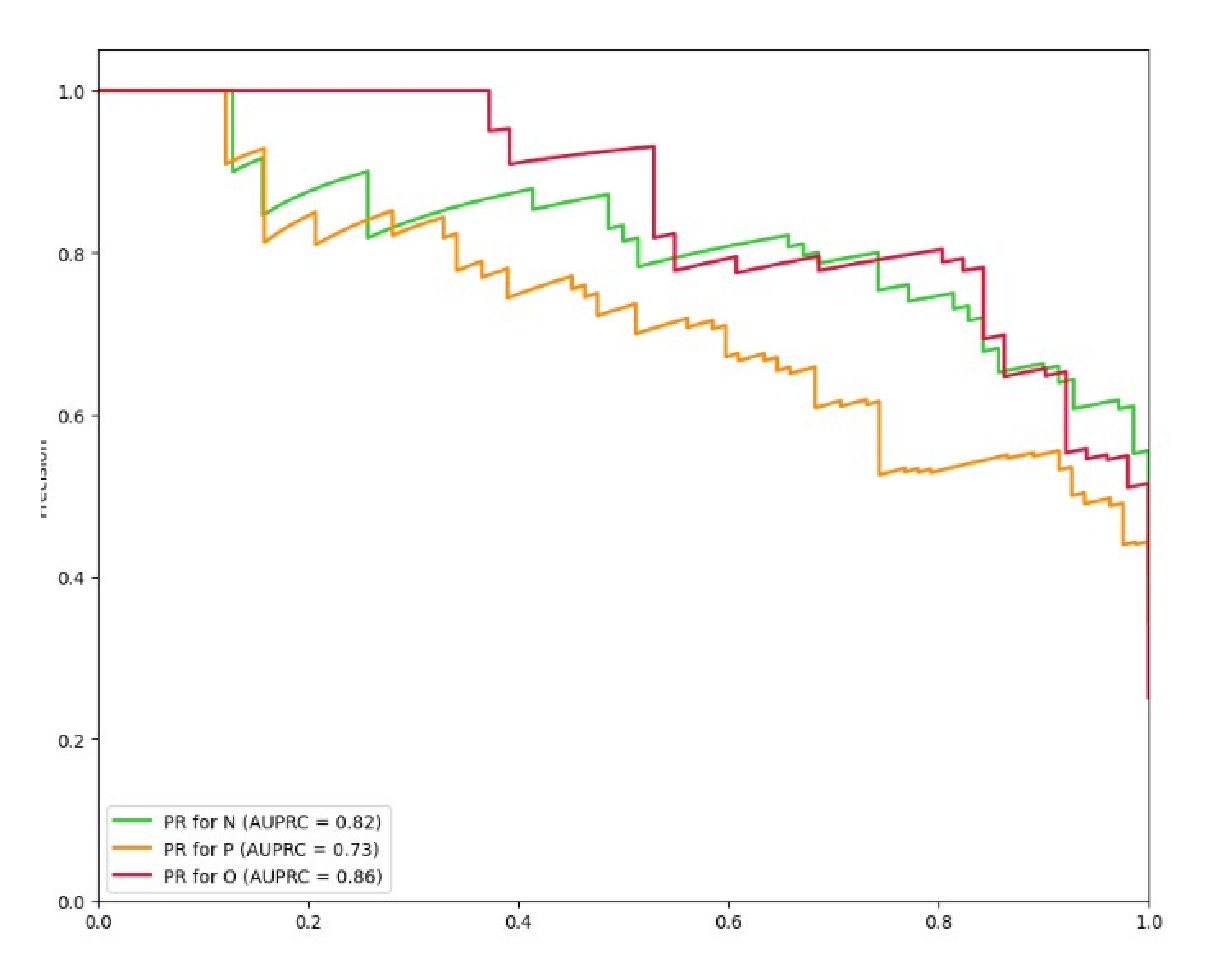
\includegraphics[width=\linewidth]{assets/pdf/Curve_PR.pdf}
\caption{Precision-Recall Curve}
\label{fig:curve_pr}
\end{figure}